\chapter{Context and objectives} \label{chapter2}
\minitoc
\eject

This chapter presents the general context for this work, and leads to a definition of the scope of this thesis.
Section \ref{chapter2:web-as-a-platform} presents the context of web development, and the motivations that led the web to become a software platform.
It presents Javascript as the main language of the web available for prototyping.
Then, it presents the problematic of developing web server past this prototyping phase for large audiences.
Section \ref{chapter2:problem-statement} states the problem tackled by this thesis, and its objectives.
The languages often fail to grow with the project they initially supported very efficiently.
The inadequacy of the languages to support the growth of web applications leads to wasted development efforts, and additional costs.
The objective of this thesis is to avoid these efforts and costs.
It intends to propose a continuous development from the initial prototype up to the releasing and maintenance of the complete product.

\section{The Web as a platform}

\subsection{From operating systems to the web}


With the invention of electronic computing machine, appeared the market for software applications.
This market is not limited by marginal production cost ; software being a virtual product, the production and distribution cost for another unit is virtually null.
The market is limited by the platform a software can be deployed on.
The bigger the platform, the wider the market.
There is an economically incentive to standardize and widen the platform, both for the provider, and for the consumer.
The first platforms started as products, in competition with other products.
Their manufacturers had economical incentive to increase their market share.
Microsoft successfully took over the market of operating system in the 90s, and was on the edge of monopoly more than once.
But eventually, the product is standardized, and becomes the platform.

\begin{wrapfigure}{r}{0.2\textwidth}
  \vspace{-27pt}
  \begin{center}
    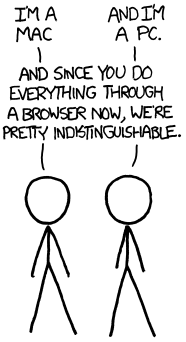
\includegraphics[width=0.18\textwidth]{../ressources/Mac-PC.png}
  \end{center}
  \vspace{-20pt}
\end{wrapfigure}

Before the internet, this market was limited for distribution by the physical medium.
It takes time to burn a CD, or a floppy, and to bring it to the consummer's home.
Sir Tim Berners Lee invented the world wide web in 1989.
It was initially intended to share scientific documents and results.
And it eventually became the distribution medium of choice for every virtual products, software included.
It pushed the scalability of software distribution.

Similarly to operating systems, Web browsers started as software products.
They exposed innovative features to try to increase their market share.
Among others is the ability to run scripts.
It allows to deploy and run software at unprecedented scales.
The web became the platform.
Now, with web services, or Software as a Service (SaaS), the distribution medium of software is so transparent that owning a software product to have an easier access is no longer relevant.
We explore now the different languages to write and deploy applications on the web.

\subsection{The languages of the web}

In the early 90's, during the web early development, most of the now popular programming languages were released.
Python(1991), Ruby(1993), Java(1994), PHP(1995) and  Javascript(1995).
With Moore's law predicting exponential increase in hardware performance, the industry realized that development time is more expensive than hardware.
Low-level languages were replaced by higher-level language, trading performance for accessibility.
The economical gain in development time compensated the worsen performances of these languages.

Java, developed by Sun Microsystems, imposes itself early as a language of choice and never really decreased.
The language is executed on a virtual machine, allowing to write an application once, and to deploy it on heterogeneous machines.
The software industry quickly adopted it as its main development language.
It is currently the second most cited language on StackOverflow, and used on Github.
And is in the first place of many language popularity indexes.
However, the software industry wants stable and safe solutions.
This prudence generally slows down Java evolution.
The language struggled to keep up with the latest trends in software development.

\textit{Python is the second best language for everything.}
It is a general purpose language, currently popular for data science.
In 2003, the release of the Django web framworks brought the language to the web development scene.

Ruby was confined in Japan and almost unknown to the world until the release of Rails in 2005.
With the release of this web framework, Ruby took-off and is still in active use.
It meets the latest trends in software development.
And it might had replaced Java if the latter had not been so well adopted in the software industry.

PHP stands for Personal Home Page Tools.
It was initially designed to build personal web pages.
It might be one of the easiest language to start web development.
However, according to several language popularity indexes, it is on a slow decline since a few years.
It is generally unfit to grow projects to industrial size.

Since a few years, Javascript is slowly becoming the main language for web development.
It is the only choice in the browser.
Because of this unavoidable position, it became fast (V8, ASM.js) and usable (ES6, ES7).
It is a target for LLVM, allowing many languages to compile to Javascript, strengthening again its omnipresent position.
Additionally, it is present on the server as well with Node.js
It is everywhere.
I argue in this thesis, that Javascript is the language of choice to bring a prototype to industrial standards.

\subsection{Explosion of Javascript popularity}

\subsubsection{In the beginning}

Javascript was created by Brendan Eich at Netscape around May 1995, and released to the public in September.
At the time, Java was quickly adopted as default language for web servers development, and everybody was betting on pushing Java to the client as well.
The history proved them wrong.

When Javascript was released in 1995, the world wide web was on the rise.\ftnt{http://www.internetlivestats.com/internet-users/}
Browsers were emerging, and started a battle to show off the best features and user experience to attract the wider public.\footnote{to get an idea of the web in 1997 : \url{http://1x-upon.com/}}
Javascript was released to be one of these features on Netscape navigator.
Microsoft released their browser Internet Explorer 3 in June 1996 with a concurrent implementation of Javascript.
At the time, because of the differences between the two implementations, web pages had to be designed for a specific browser.
This competition was fragmenting the web.

Netscape submitted Javascript to Ecma International for standardization in November 1996 to stop this fragmentation.
In June 1997, ECMA International released ECMA-262, the first specification of ECMAScript, the standard for Javascript.
A standard to which all browser should refer for their implementations.
% TODO more on the Ecma specification ?

The initial release of Javascript was designed in a rush. The version released in 1995 was finished within 10 days.
And, it was intended to be simple enough to attract unexperienced developers.
For these reasons, the language was considered poorly designed and unattractive by the developer community.

But things evolved drastically since.
The success of Javascript is due to many factors ; maybe the most important of all is the \textit{View Source} menu that reveals the complete source code of any web application.
\textit{The view source menu is the ultimate form of open source}\ftnt{http://blog.codinghorror.com/the-power-of-view-source/}.
It is the vector of the quick dissemination of source code to the community, which picks, emphasizes and reproduces the best techniques.
It brought open source and collaborative development to the web.
Moreover, all web browsers include a Javascript interpreter, making Javascript the most ubiquitous runtime in history \cite{Flanagan2006}.
% Every browser include development tools for Javascript, making it the most ubiquitous development environment, as well.

When such a language is distributed freely with the tools to reproduce and experiment on every piece of code.
And its distribution is carried during the expansion of the largest communication network in history.
Then an entire generation seizes this opportunity to incrementally build and share the best tools they can.
This collaboration is the reason for the popularity of Javascript on the Web.
% When a language is released, available freely at a world wide scale, and simple enough to be handled by a generation of teenager inspired by the technology hype, it produce an effervescent community around what is now one of the most popular and widely used programming language.

\subsubsection{Rising of the unpopular language}

\begin{figure}[h!]
{\fontfamily{phv}\fontseries{l}
\fontsize{10pt}{10pt}\selectfont
Why does Javascript suck?\ftnt{http://whydoesitsuck.com/why-does-javascript-suck/}

Is Javascript here to stay?\ftnt{http://www.javaworld.com/article/2077224/learn-java/is-javascript-here-to-stay-.html}

Why Javascript Is Doomed.\ftnt{http://simpleprogrammer.com/2013/05/06/why-javascript-is-doomed/}

Why JavaScript Makes Bad Developers.\ftnt{https://thorprojects.com/blog/Lists/Posts/Post.aspx?ID=1646}

JavaScript: The World's Most Misunderstood Programming Language\ftnt{http://www.crockford.com/javascript/javascript.html}

Why Javascript Still Sucks\ftnt{http://www.boronine.com/2012/12/14/Why-JavaScript-Still-Sucks/}

10 things we hate about JavaScript\ftnt{http://www.infoworld.com/article/2606605/javascript/146732-10-things-we-hate-about-JavaScript.html}

Why do so many people seem to hate Javascript?\ftnt{https://www.quora.com/Why-do-so-many-people-seem-to-hate-JavaScript}
}
\end{figure}

Javascript started as a programming language to implement short interactions on web pages.
The best usage example was to validate some forms on the client before sending the request to the server.
This situation hugely improved since the beginning of the language.
Nowadays, there is a lot of web-based application replacing desktop applications, like mail client, word processor, music player, graphics editor…

There is now more software services released to the public as web-based application compared to desktop clients.

ECMA International released several version in the few years following the creation of Javascript.
The first and second version, released in 1997 and 1998, brought minor revisions to the initial draft.
However, the third version, released in the late 1999, contributed to give Javascript a more complete and solid foundation as a programming language.
From this point on, the consideration for Javascript kept improving.

%An important reason for this reconsideration started in 2005.
In 2005, James Jesse Garrett released \textit{Ajax: A New Approach to Web Applications}, a white paper coining the term Ajax \cite{Garrett2005}.
This paper points the trend in using this technique, and explain the consequences on user experience.
Ajax stands for Asynchronous Javascript And XML.
It consists of using Javascript to dynamically request and refresh the content inside a web page.
It has the advantage to avoid requesting a full page from the server.
Javascript is not anymore confined to the realm of small user interactions on a terminal.
It can be proactive and responsible for a bigger part in the whole system spanning from the server to the client.
Indeed, this ability to react instantly to the user gave to developer the feature to develop richer applications inside the browser.
%, while keeping all the advantages of web-based applications.
At the time, the first web applications to use Ajax were Gmail, and Google maps\footnote{A more in-depth analysis of the history of Ajax, given by late Aaron Swartz \url{http://www.aaronsw.com/weblog/ajaxhistory}}.

Around this time, the Javascript community started to emerge.
The third version of ECMAScript had been released, and it was homogeneously supported in the browsers.
However, the DOM, and the \texttt{XMLHttpRequest} method, two components on which AJAX relies, still present heterogeneous interfaces among browsers.
Javascript framework were released with the goal to straighten the differences between browsers implementations.
Prototype\ftnt{http://prototypejs.org/} and DOJO\ftnt{https://dojotoolkit.org/} are early famous examples, and later jQuery\ftnt{https://jquery.com/} and underscore\ftnt{http://underscorejs.org/}.
These frameworks are responsible in great part to the wide success of Javascript and of the web technologies.

In the meantime, in 2004, the Web Hypertext Application Technology Working Group\ftnt{https://whatwg.org/} was formed to work on the fifth version of the HTML standard.
This new version provide new capabilities to web browsers, and a better integration with the native environment.
It features geolocation, file API, web storage, canvas drawing element, audio and video capabilities, drag and drop, browser history manipulation, and many mores.
It gave Javascript the missing interfaces to become a rich environment to develop rich application in the browser.
The first public draft of HTML 5 was released in 2008, and the fifth version of ECMAScript was released in 2009.
These two releases, ECMAScript 5 and HTML5, represent a mile-stone in the development of web-based applications.
Javascript became the programming language of this rising application platform.

Javascript, and web technologies are also used outside the web.
NW.js\ftnt{https://github.com/nwjs/nw.js} and electron\ftnt{https://github.com/atom/electron} are two solutions to deploy application built with web technologies.
They use Node.js and Chromium.
The Atom text editor\ftnt{https://atom.io/}, Popcorn Time\ftnt{https://popcorntime.io/} and Light Table\ftnt{http://lighttable.com/} are example of such applications.
However, if web applications are common choice for web service client on the desktop, HTML5 is not yet widely accepted as ready to build complete application on mobile, where performance and design are crucial.
Indeed web-technologies are often not as capable, and well integrated as native technologies.
But even for native development, Javascript seems to be a language of choice.
An example is the React Native Framework\ftnt{https://facebook.github.io/react-native/} from Facebook, which allow to use Javascript to develop native mobile applications.
They prone the philosophy \textit{"learn once, write anywhere"}, in opposition to the usual slogan \textit{"write once, run everywhere"}.\footnote{Used firstly by Sun for Java, but then stolen by many others}
% Another example is Gnome-shell. It uses Javascript to build its interface, and extensions.
% PhoneGap (Cordova) is a huge effort toward bringing web technologies to the mobile.

\nt{Insert in this section a summary table for HTML and Javascript}

\subsubsection{Current situation}

\cit{When JavaScript was first introduced, I dismissed it as being not worth my attention. Much later, I took another look at it and discovered that hidden in the browser was an excellent programming language.}{Douglas Crockford}

% \cit{JavaScript is the world's most ubiquitous computing runtime.}{John Lam}



% I want to say that Javascript took off because it was carried by the open source community.
% The goal is to introduce the following facts : JS is widely used in the open source community.
% I need to find the argument saying that open source is taking over closed sources : Javascript / open source is taking over Java / closed source.

% TO READ :
% http://www.javaworld.com/article/2077224/learn-java/is-javascript-here-to-stay-.html
% http://blog.codinghorror.com/the-power-of-view-source/
% http://blog.codinghorror.com/javascript-the-lingua-franca-of-the-web/
% http://shaver.off.net/diary/2007/05/10/the-high-cost-of-some-free-tools/


% This success is obvious on the web and in the open source communities.
The rise of Javascript is obvious on the web and particularly the open source communities.
It also seems to be rising in the software industry.
However, it is harder to give an accurate picture of the situation.
The software industry is not as clear and open as the web.
Moreover, there is no right metrics to accurately and directly measure programming language popularity.
In the following paragraphs, I report some of the best metrics and indexes available freely on the web to try to represent the situation, both in the open source community and in the more opaque software industry.
More detailed informations are available section \ref{appendix:langpop}.

\paragraph{Available resources}

The TIOBE Programming Community index is a monthly indicator of the popularity of programming languages.
Javascript ranks 6th on this index, as of April 2015, and it was the most rising language in 2014.
It uses the number of results on many search engines as a measure of the popularity of a programming language.
The results contains learning and training resources, forums logs, books and many other traces of the activity of a the community around the language.
However, the measure used by the TIOBE is controversial, and might not be representative.
It is a lagging indicator, and the number of pages doesn't represent the number of readers.

Alternatively, the PYPL index is based on Google trends to measure the number of requests on a programming language.
Javascript ranks 7th on this index, as of May 2015.
This index seems to be more accurate, as it depicts the actual interest of the community for a language.
However, it is not representative as it only takes Google search into account.

From these indexes, the major programming languages are Java, C/C++ and C\#.
The three languages are still the most widely taught, and used to write softwares.
But Javascript is rising to become an important language as well.

\paragraph{Developers collaboration platforms}

An indicator of the popularity and usage of a language is the number of developers and projects using it.

Github is the most important collaborative development platform, with around 9 millions users.
Javascript is the most used language on github since mid-2011, with more than 320 000 repositories.
The second language is Java with more than 220 000 repositories.

\nt{TODO : graph of Github repositories by languages}

StackOverflow, is the most important Q\&A platform for developers.
It is a good representation of the activity around a language.
Javascript is the second language showing the most activity on StackOverflow, with more than 840 000 questions.
The first one is Java with more than 850 000 questions.

Black Duck Software helps companies streamline, safeguard, and manage their use of open source.
For its activity, it analyzes 1 million repositories over various forges, and collaborative platforms to produce an index of the usage of programming language in open source communities.
Javascript ranks second.
C is first, and C++ third.
Along with Java, the four first languages represent about 80\% of all programming language usage.

\nt{TODO redo this graph, it is ugly.}
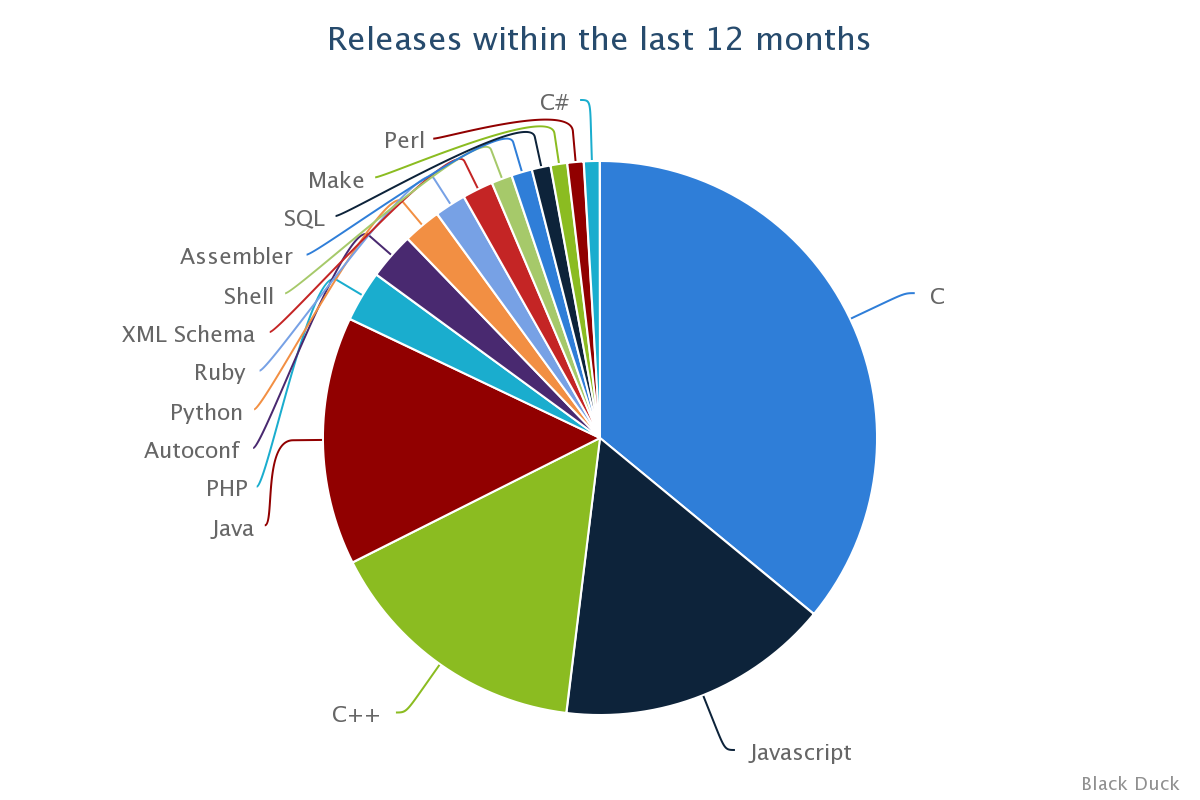
\includegraphics[width=0.9\linewidth]{../../data/js-trends/black-duck-15}

% \begin{figure}[h!]
% \begin{tikzpicture}
% [
%     pie chart,
%     slice type={c}{gray1},
%     slice type={js}{red},
%     slice type={cpp}{gray2},
%     slice type={java}{gray3},
%     slice type={php}{gray4},
%     slice type={autoconf}{gray5},
%     slice type={python}{gray6},
%     slice type={ruby}{gray1},
%     slice type={xml}{gray2},
%     slice type={sh}{gray3},
%     slice type={asm}{gray4},
%     slice type={sql}{gray5},
%     slice type={make}{gray6},
%     slice type={perl}{gray1},
%     slice type={csharp}{gray2},
%     pie values/.style={font={\small}},
%     scale=2
% ]

% \pie{}{%
%   34.80/c,%
%   15.45/js,%
%   15.13/cpp,%
%   14.02/java,%
%   2.87/php,%
%   2.65/autoconf,%
%   2.15/python,%
%   1.77/ruby,%
%   1.73/xml,%
%   1.18/sh,%
%   1.16/asm,%
%   1.07/sql,%
%   0.94/make,%
%   0.92/perl,%
%   0.90/csharp,%
% }

% \legend[shift={(1.3cm,0.9cm)}]{%
%   {C}/c,%
%   {Javascript}/js,%
%   {C++}/cpp,%
%   {Java}/java,%
%   {PHP}/php,%
%   {Autoconf}/autoconf,%
%   {Python}/python,%
%   {Ruby}/ruby,%
%   {XML Schema}/xml,%
%   {Shell}/sh,%
%   {Assembler}/asm,%
%   {SQL}/sql,%
%   {Make}/make,%
%   {Perl}/perl,%
%   {C\#}/csharp,%
% }
% \end{tikzpicture}
% \caption{Compilation results distribution}
% \end{figure}

\paragraph{Jobs}

The software industry is rather closed sourced, and its activity is rather opaque.
All these previous metrics are representing the visible activity about programming language, but are not representative of the software industry.
%To get a hint on the popularity of programming languages used in the software industry, the trends on job propositions are insightful.
The trends on job openings gives an hint of the direction the software industry is heading towards.
\textit{Indeed} provide some trends over its database of job propositions.
Javascript developers ranked at the third position, right after SQL and Java developers.
Then come C\# and C developers.
This position means that Javascript might finally be on the edge to become a major language in the software industry, and become as important as Java and C/C++.

\nt{TODO redo this graph, it is ugly.}
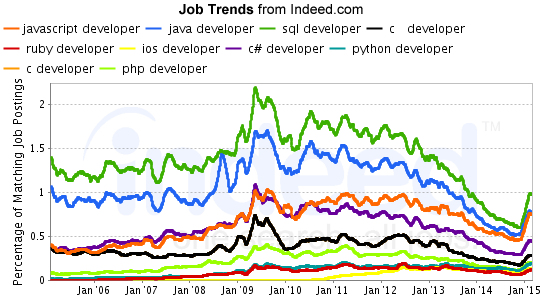
\includegraphics[width=0.9\linewidth]{../../data/js-trends/jobgraph}



All these metrics in this section represent different faces of the current situation of Javascript adoption.
With the rise of web applications, we can safely say that Javascript is one of most important language of this decade, alongside with Java and C/C++.
It is widely used in open source projects, and everywhere on the web, as well as in the software industry.
\section{An Economical Problem} \label{chapter2:problem-statement}

With Software as a Service (SaaS), the software industry is in charge of both development and execution of the software.
The previous section presented these two aspects individually.
This section presents the challenges encountered by conducting the two at world wide scale.
It then focuses on the subject of this thesis and defines its objectives.

\subsection{Disrupted Web Development}

The economical constraints to meet are very different in the beginning and during the maturation of a web application.
In the early steps the constraints hold on the development productivity.
The team needs to reduce development costs, and to release a first version as soon as possible.
On the contrary, during the maturation of the application, the constraints hold on the performance efficiency.
The application needs to be highly concurrent to meet the load of usage.

The team needs to revise its approach to meet these different constraints.
Which leads to disruptions in the evolution of the application.

\subsubsection{Power-Wall Disruption}

\marginfig{10}{0.5\textwidth}{
  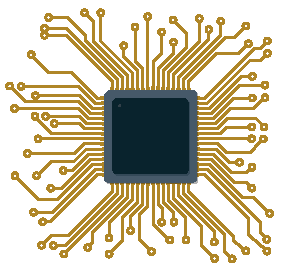
\includegraphics[width=0.3\textwidth]{../resources/chip.pdf}%
}

Around 2004, manufacturers reached what they called the \textit{Power-wall}.
The speed of sequential execution on a processing unit plateaued\ftnt{http://bit.ly/dennard-scaling}.
Therefore, the performance of sequential programming plateaued as well.
They started to arrange transistors into several processing units to keep increasing overall performance efficiency.
Parallel programming became the only option to achieve high concurrency, but the memory isolation it requires limits the productivity.
This \textit{Power-wall} leads to a rupture between efficiency and productivity.

\subsubsection{Conflicting Modularity}

The best practices for productivity in software development advocate to gather features logically into distinct modules.
This modularity allows a developer to understand and contribute to an application one module at a time, instead of understanding the whole application.
It allows to develop and maintain a large code-base by a multitude of developers bringing small, independent contributions.

This modularity avoids a different problem than the isolation required by parallelism.
The former intends to structure code to improve maintainability, while the latter improves performance through parallel execution.
These two organizations are conflicting in the design of the application.
The next paragraph presents the disruptions in the development of a web application implied by this conflict.

\subsubsection{Technological Shift}

% Between the prototyping, and the maturation of a web application, the needs are radically different.
% During the initiation of a web application project, the economical constraint holds on the development productivity.
% The development reactivity is crucial to meet the market needs\ftnt{https://www.cbinsights.com/blog/startup-failure-post-mortem/}.
The development team opt for a popular and accessible language to be productive in the beginning of the project. %  leverage the advantage of its community.
It is only after a certain threshold of user load that the economical constraint on efficiency exceeds the one on productivity.
The development team then shifts to an organization providing parallelism.

This shift brings two risks.
The development team needs to rewrite the code base to adapt it to a completely different paradigm.
The application risks to fail because of this challenge.
And after this shift, the development is less productive.
The development team cannot react as quickly to user feedbacks to adapt the application to the market needs.
The application risks to fall in obsolescence.

The risks implied by this rupture proves that there is economically a need for a solution that continuously follows the evolution of a web application.
The solution proposed in this thesis would allow developers to iterate continuously on the implementation focusing continuously on maintainability and performance.

\subsection{Seamless Web Development}

This thesis is conducted in the frame of a larger work on LiquidIT within the Worldline company.
Worldline develops and hosts real-time streaming Web services.
The company identified that one of its need was to increase the time to market for its products.
Worldline defines LiquidIT as \textit{a concept of flexible and cost-effective IT services that can be provisioned, built and configured in real time, allowing end-to-end financial transparency}.
It precisely intends to provide \textit{business agility, investment-free charging models, flexibility and ease of use}.
This thesis intends to allow the developer to focus solely on business logic, and leave the technical constraints of performance scalability to automated tools.
The objective of this work are to avoid the disruption in development, and provide a seamless development experience.
% They are presented in the next paragraphs.

\subsubsection{Real-Time Streaming Web Services}

This thesis focuses on web applications processing streams of requests from users in soft real-time.
Such applications receive requests from clients through the HTTP protocol and must respond within a finite window of time.
They are generally organized as sequences of tasks to modify the input stream of requests to produce the output stream of responses.
The stream of requests flows through the tasks, and is not stored.
On the other hand, the state of the application remains in memory to impact the future behaviors of the application.
This state might be shared by several tasks within the application, and imply coordination between them.

As presented in the previous section, such applications are often implemented with the event-driven programming model or the pipeline programming model.
This thesis develops an equivalence to map these two models, despite their differences.
% The next section introduces the differences between these two programming models and outlines an equivalence to map these differences.

\subsubsection{Differences Between The Two Models}

Both programming models encapsulate the execution in tasks assured to have an exclusive access to the memory.
However, they use two different models to provide this exclusivity.
Contrary to the pipeline architecture, the event-loop provides a common memory store allowing the best practice of software development to improve maintainability.

These two organizations are incompatible.
And because of economical constraints, this incompatibility implies ruptures in the development.
It represents additional development efforts and important costs.
This thesis argues that it is possible to allow a continuous development between the two organizations, so as to lift these efforts and costs.
To do so, it proposes an equivalence between the two organizations to change from one into the other.
% The argumentation of this possibility is based on an equivalence bridging the two organizations.
It briefly introduces this equivalence in the next paragraph, and details it further in the chapter \ref{chapter4} and \ref{chapter5}.

\subsubsection{Equivalence}

In the beginning of a project, the team focus on productivity, maintainability and evolution, discarding the scalable performance concerns.
The team adopts the event-driven execution model and always sticks with the productive model.
And as the project gather audience and the performance concerns become more and more critical.
The equivalence allows to transform an application expressed in the event-driven execution model into the pipeline execution model.
The generated pipeline expression allows the execution engine to adapt itself to any parallelism of the computing machine, from a single core, to a distributed cluster.
Without giving the productive model up, the development team takes advantage of the different concerns of the tow execution model, performance and maintainability.

\separator

This thesis proposes to provide an equivalence between the two memory models for streaming web applications.
The goal of conciliating these two concerns is not new.
The next chapter presents all the previous results needed to understand this work, up to the latest advances in the field.